\lstinputlisting[language=Matlab]{cap_2/es7/es7.m}

I dati generati dall'esecuzione del codice sono esposti  nella seguente tabella

\begin{tabular}{|l|c|c|}
\hline
$n$ & $tol_x$ & $y$ \\
\hline
0 & $10^{-1}$ & 0.500000000000000 \\
7 & $10^{-2}$ & 0.488281250000000 \\
10 & $10^{-3}$ &  0.488769531250000 \\
13 & $10^{-4}$ & 0.488952636718750 \\
16 & $10^{-5}$ & 0.488945007324219 \\
20 & $10^{-6}$ & 0.488943576812744 \\
21 & $10^{-7}$ & 0.488943815231323 \\
26 & $10^{-8}$ & 0.488943792879581 \\
30 & $10^{-9}$ & 0.488943794276565 \\
32 & $10^{-10}$ & 0.488943794392981 \\
\hline
\end{tabular}\\
\begin{figure}[b]
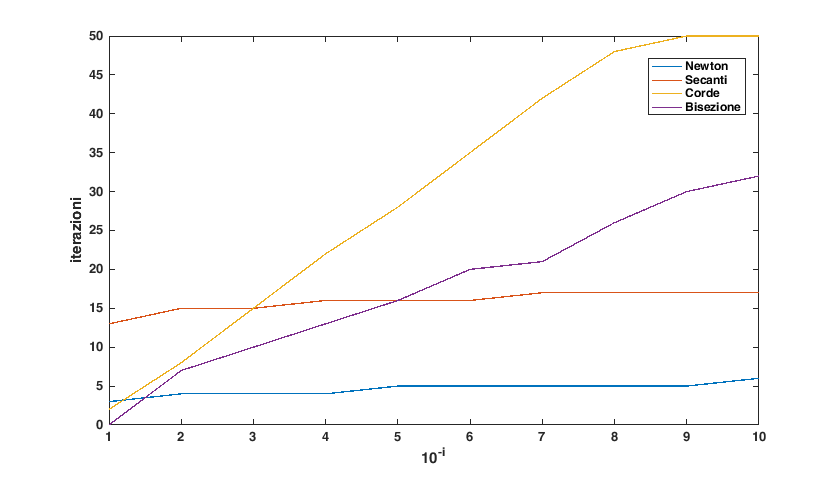
\includegraphics[scale=0.7]{cap_2/es7/compar}
\caption{Comparazione del numero di iterazioni necessarie per i vari metodi}
\label{compar}
\end{figure}
Per la comparazione vedi figura \ref{compar}
